\documentclass[10pt, oneside]{article} 

\usepackage{amsmath, amsthm, amssymb,amsfonts,appendix}
\usepackage{bbm, bm,booktabs}
\usepackage{calrsfs,color,cite,caption}
\usepackage{esint,enumitem}
\usepackage{fancyhdr,fontspec,float}
\usepackage{graphicx,graphics,geometry}
\usepackage{hyperref}
\hypersetup{
    colorlinks=true,
    linkcolor=blue,
    filecolor=blue,      
    urlcolor=blue,
    citecolor=blue,
}
\usepackage{indentfirst}
\usepackage[labelfont=bf]{caption}
\usepackage{mathptmx}
\usepackage{stmaryrd,siunitx,subfigure,setspace}
\usepackage[stable]{footmisc}
\usepackage{tikz,textcomp}
\usetikzlibrary{fit,positioning,arrows,automata}
\usepackage{verbatim}
\usepackage{wasysym}
\usepackage{wrapfig}



\geometry{tmargin=.75in, bmargin=.75in, lmargin=.75in, rmargin = .75in}  



\newtheorem{thm}{Theorem}
\newtheorem{defn}{Definition}
\newtheorem{conv}{Convention}
\newtheorem{rem}{Remark}
\newtheorem{lem}{Lemma}
\newtheorem{cor}{Corollary}


\title{
Independent Study Final Report\\
\Large Automatic Music Generation \\
}
\author{Yuheng Ma\\[0.3cm]{ Mentor: Sayan Mukherjee, Anna Yanchenko}}
\date{Fall 2019}

\begin{document}

\maketitle

\vspace{.25in}

\section{Introduction}
Automatic music generation, which means a process of using some formal process to make music with minimal human intervention\cite{briefhistoryofac}, has centuries of history. An early example is Dice Music by Wolfgang Amadeus Mozart\cite{algorithmiccomposition} in the 18th century, a game that involved assembling a number of small musical fragments and combining them randomly, piecing together a new piece. A notably wide range of methods are implemented in algorithmic composition with the help of computers. A well-known early work on algorithmic composition was the Illiac Suite that utilized the classical rules for counterpoint in the generation of the first and second movements (Hiller \& Isaacson, 1958)\cite{AImethodsinalgorithmicomposing}. Since 2016, Google's Magenta\cite{magenta} has been exploring the role of neural networks and deep learning  in the process of creating art and music. Hidden Markov Models (HMMs) are a statistical model that have been utilized in many aspects of music analysis and generation. Farbood and Schoner (2001) \cite{farbood2001analysis} were the first to apply HMMs to composition with fixed melody patterns. This report is a part of the future work of Anna Yanchenko's\cite{yanchenko2017classical}, which explored application of variations of HMMs and time varying autoregression models in algorithmic composition of piano pieces in the Romantic era, focusing especially on melody.

The main goal of this work is to apply a variation of HMMs called a first order dilated convolution to compose piano pieces and evaluate the generated pieces' quality with respect to different targets. We also train on multiple input sequences as a way to average the influence of a single piece and modify a style in general. Some results give confirmation to the intuition of the model, while some results remain to be further explored.


\section{Data and Processing}
To learn from input pieces and return generated pieces, the algorithm will need a digital representation of music, which carries information about pitch, velocity, clock signal, etc. A common format is the Musical Instrument Digital Interface (MIDI) \cite{midiwiki}. However, if we directly use MIDI and regard all possible note and velocity combinations at each time signature as the state space, there will be too many possibilities. Thus, underfitting may happen and the model will take more time to run. Also, it's not reasonable to combine notes and velocities since there is no direct relevance between. To be compatible with HMMs, the MIDI representation is transferred into a sequence of note pitches (either one note or chords) at discrete time intervals, represented by one of finitely many positive integers. This allows the modeling of notes directly by the HMMs. For the single dilated convolution model, we simply take exactly the same timing information from the original piece. For the models trained on multiple sequences, timing information is randomly sampled from the original pieces. The velocities are interpolated and not modeled directly. These together form a generated piece.

In order to adopt the multiple sequences method, several pieces in a similar composing style are required. 
The input pieces for this report are 20 piano pieces, listed in Appendix \ref{appendix:b}. These are all originally MIDI files, transformed to a CSV file  \cite{midicsv} and then processed to sequences of integer notes \cite{annagithub}. 
\section{Model}
The new model and its multiple input version are derived from the standard first order HMM.


$\mathbf{First \;Order\;HMM}$
Denote the length of a sequence as T, observation sequence and latent sequence as $\{ X_1,\cdots, X_T\}:=X_{1:T}$, $\{ Z_1,\cdots, Z_T\}:=Z_{1:T}$. Then the likelihood for the regular HMM is
$$
P\left(X_{1: T}, Z_{1: T}| A, b, \pi \right)=P\left(Z_{1}| \pi \right) P\left(X_{1} | Z_{1}, b \right) \prod_{t=2}^{T} P\left(Z_{t} | Z_{t-1}, A\right) P\left(X_{t} | Z_{t},b\right)
$$
where $A$ represents the transition probability, $b$ represents the emission probability and $\pi$ represents the initial distribution. The expectation maximization algorithm, which is used to optimize the parameters, is the Baum-Welch algorithm.\cite{tutorial}\\

$\mathbf{Dilated\; Convolution}$
Some interpretable variations can be made based on features of music. Besides an approximate distribution of notes and chords, we also want the model to grab some long-term structure, such as motifs. In the regular HMM, the previous latent states influence the next observation through the next latent state  by determining the latent distribution and then the emission distribution. We can allow a direct influence between the previous hidden state and the current observation to improve the effect of a short past. The graphical model is as follows. 

\begin{figure}[!htb]\centering
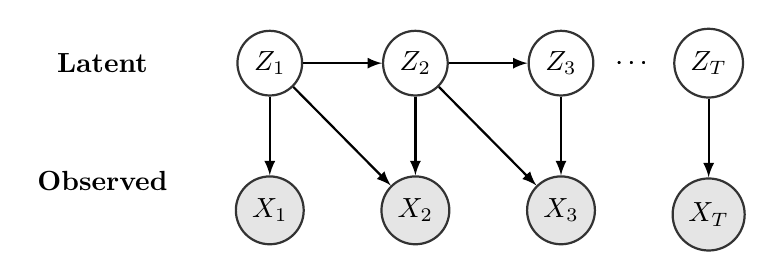
\begin{tikzpicture}
\tikzstyle{main}=[circle, minimum size = 5mm, thick, draw =black!80, node distance = 10mm]
\tikzstyle{connect}=[-latex, thick]
\tikzstyle{box}=[rectangle, draw=black!100]
  \node[box,draw=white!100] (Latent) {\textbf{Latent}};
  \node[main] (L1) [right=of Latent] {$Z_1$};
  \node[main] (L2) [right=of L1] {$Z_2$};
  \node[main] (L3) [right=of L2] {$Z_3$};
  \node[main] (Lt) [right=of L3] {$Z_T$};
  \node[box,draw=white!100] (Observed) [below=of Latent] {\textbf{Observed}};
  \node[main,fill=black!10] (O1) [right=of Observed,below=of L1] {$X_1$};
  \node[main,fill=black!10] (O2) [right=of O1,below=of L2] {$X_2$};
  \node[main,fill=black!10] (O3) [right=of O2,below=of L3] {$X_3$};
  \node[main,fill=black!10] (Ot) [right=of O3,below=of Lt] {$X_T$};
  \path (L3) -- node[auto=false]{\ldots} (Lt);
  \path (L1) edge [connect] (L2)
        (L2) edge [connect] (L3)
        (L3) -- node[auto=false]{\ldots} (Lt);
  \path (L1) edge [connect] (O1);
  \path (L2) edge [connect] (O2);
  \path (L3) edge [connect] (O3);
  \path (Lt) edge [connect] (Ot);
  \path (L1) edge [connect] (O2);
  \path (L2) edge [connect] (O3);
  \draw[dashed]  [below=of L1,above=of O1];
\end{tikzpicture}
\end{figure}

The model is called $\mathbf{Dilated\;Convolution\;(first \;order)}$. We are expecting a better performance of this model in grabbing a long-term pattern. The likelihood function for this model is 
$$
P\left(X_{1: T}, Z_{1: T}| A, b, \pi \right)=P\left(Z_{1}| \pi \right) P\left(X_{1} | Z_{1}, b \right) \prod_{t=2}^{T} P\left(Z_{t} | Z_{t-1}, A\right) P\left(X_{t} | Z_{t-1},  Z_{t},b\right)
$$
The expectation maximum algorithm for this model is given in Appendix \ref{appendix:c}.\\

$\mathbf{Multiple\; Input}$
In order to have sufficient data to make a reliable estimate of the parameters, we may consider learning from multiple observation sequences. The joint likelihood is 
$$
P(X^{1}_{1:T},\cdots, X^{K}_{1:T},Z_{1:T})=\prod_{k=1}^{K} P(X^{k}_{1:T}, Z_{1:T})
$$
The expectation maximum algorithm for this model is in Appendix \ref{appendix:d}.

We consider 4 models in total. First, we generate from the dilated convolution model with 5 hidden states and 10 hidden states respectively. Then, we apply the multiple input version. All of these models are compared with the standard first order HMM.

\section{Result}
\subsection{Evaluation Metrics }
The metrics we used in the following section are to evaluate the performance of generated pieces  by Romantic style criterion in the sense of originality, musicality and temporal structure. The originality tells about the relevance between generated and original pieces, as well as complexity of generated pieces. Empirical entropy, edit distance and mutual information are considered. Musicality metrics include counts of notes, dissonant harmonic intervals and melodic intervals, all normalized by the length of the piece. We also use the percentage of intervals that are perfect consonances, imperfect consonances and dissonances. For temporal structure, PACF and ACF are considered as metrics that represent the decay correlation of the system. 

After learning and optimizing the parameters by Baum-Welch, 1000 new pieces are generated. Each metric of the algorithm (except mutual information and edit distance ) RMSE is used to compare the generated pieces to the original piece. For mutual information and edit distance, we take their average over all generated pieces.
\subsection{Dilated Convolution Single Input}
For the single input version, we take ``Pachelbel's Canon" as an example and set the number of hidden states to 5 as the default. As previously mentioned, the intuition of the dilated convolution model is to grab a longer-term structure. As a result, we focus on the ACF/PACF metrics, which can reflect whether sequences have a high degree of global structure. The expected ACF/PACF plot of the dilated convolution model would have structure to higher lags than the first order plot.
\begin{figure}[H]

  \includegraphics[width=\linewidth]{ACF.png}

  \label{fig: ACF}
    \caption{ACF/PACF plot for first order and dilated convolution training on Pachelbel.}
\end{figure}

From \hyperref[fig: ACF]{Figure 1}, the dilated convolutions model shows some persistence in ACF/PACF, but it's not sufficient to draw the conclusion that this modification of the first order model leads to better global structure. 
The other calculated metrics are listed in \hyperref[table:metrics]{Table 1}. 
\\

\begin{table}[!htbp]
\centering
\begin{tabular}{|l|l|l|l|l|l|l|l|}
\hline
                                                                        & Entropy & Mutual Info & Edit    & H Intervals  & M Intervals  & Percent & Note Count \\ \hline
\begin{tabular}[c]{@{}l@{}}First-Order\\ Pachelbel\end{tabular}         & 0.04029 & 0.33813     & 0.87228 & 68.16021 & 94.17695 & 0.16198 & 0.00829     \\ \hline
\begin{tabular}[c]{@{}l@{}}Dilated-Convolution\\ Pachelbel\end{tabular} & 0.02361 & 0.33659     & 0.87317 & 68.90035 & 95.73763 & 0.16175 & 0.00614     \\ \hline
\end{tabular}
\caption{Top metrics trained from Pachelbel. Metrics are successively empirical entropy, mutual information, edit distance, count of harmonic intervals normalized by piece length, count of harmonic intervals normalized by piece length, percentage of intervals and count of notes. }
\label{table:metrics}
\end{table}

From the table, we can see that the dilated convolution model generally does not outperform the first order model or is sometimes even worse. The metrics that are relatively significant are empirical entropy and the count of harmonic intervals. This is reasonable since the dilated convolution model tends to generate a system with less freedom. Meanwhile, the result in \hyperref[table:compare]{Table 2} illustrates that the comparison of results depend not only on the model but also on the original training pieces.  Thus, we should compare results across multiple input sequences. Also, a promising future work could explore the relationship between the properties of the original pieces and the metric performance of the generated pieces, which would eventually answer the question about what kind of Romantic era pieces are best to learn from. 
\\

\begin{table}[!htbp]
\centering
\begin{tabular}{|c|c|c|c|c|c|c|c|}
\hline
                                                                         & Entropy & Mutual Info & Edit    & H Intervals  & M Intervals  & Percent & Note Count \\ \hline
\begin{tabular}[c]{@{}l@{}}First-Order\\ Ode-to-Joy\end{tabular}         & 0.03283 & 0.16695     & 0.71798 & 22.15956 & 36.73144 & 0.13401 & 0.00943     \\ \hline
\begin{tabular}[c]{@{}l@{}}Dilated-Convolution\\ Ode-to-Joy\end{tabular} & 0.02930  & 0.16639     & 0.69042 & 22.14071 & 36.90521 & 0.13417 & 0.00876     \\ \hline
\end{tabular}
\caption{Top metrics trained from Ode to joy.}
\label{table:compare}
\end{table}


\newpage
$\mathbf{Interpretation}$
The hidden states have specific meanings representing the underlying dynamics of the piece. We can decompose the notes into single pitches and look at the emission matrix (the emission matrix of the dilated convolution model is three dimensional with entries $b_{ijk}=p(P_t=k|Z_{t-1}=i,Z_t=j)$ where $P_t$ is some pitch, so we fix the second index j). For instance, if a hidden state only has high emission distribution of (C) and (G), then the state catch the perfect fifth. As is shown in \hyperref[fig:inter]{Figure 2}, fixing $Z_{t-1}=0$, the hidden states 1 catches D3, 2 catches G chord, 3 catches Gmaj 7 and 4 catches A2. This means that the dilated convolution model is able to recover basic aspects of harmony, even though there is no prior harmonic musical knowledge imparted in the model.
\begin{figure}[H]
\centering

  \includegraphics[width=\linewidth]{interpretion.png}
  \caption{Emission distribution of pitches fixing $Z_{t-1}$=0}
  \label{fig:inter}
\end{figure}

\subsection{Dilated Convolution Multiple Input}
$\mathbf{Difference\; in\; Metric\; Calculation}$
When calculating metrics, edit distance and mutual information require that two pieces are compared that have the same length. Different timing information was randomly assigned to the generated pieces. Thus, the edit distance and mutual information metrics for each generated piece are calculated with the corresponding original piece. Due to the large scale of the data, we calculate the KL-divergence between the distribution of metrics on the original pieces and on all generated pieces for the other metrics. \\



$\mathbf{Label\;Switching}$
The Baum-Welch algorithm for multiple input pieces takes the weighted average of each set of parameters trained from one original pieces. However, directly doing so might ruin the subtle structure that we already have before averaging. Because of randomness of the initial value, even if the hidden states capture the same thing, the transition matrix might look completely different. For example, if five hidden states catch successively the perfect fifth, sixth chord, seventh chord, ninth chord and eleventh chord, it's unreasonable to average this transition matrix with another one which captures the sixth chord, seventh chord, ninth chord, eleventh chord and perfect fifth. 

A resolution lies in finding a permutation of the hidden states. One way is to fix one transition matrix and permute the others such that each of has the minimum distance to the reference matrix. Alternatively, we can reorder the hidden states such that the first has the highest probability in the latent sequence, and the last hidden state has the lowest probability. Then averaging all parameters seems reasonable. 


The calculated metrics are listed in \hyperref[table: multiple metrics]{Table 3}. 


\begin{table}[H]
\centering
\begin{tabular}{|c|c|c|c|c|c|c|}
\hline
           & Entropy & Harmonic Intervals & Melodic Intervals & Percent & ACF    & PACF   \\ \hline
HMM-5      & 11.0815 & 3.0508  & 4.0215  & 8.054   & 4.9671 & 2.5001 \\ \hline
HMM-10     & 11.0815 & 3.0172  & 3.9405  & 7.8203  & 5.1167 & 2.4965 \\ \hline
Dilated-5  & 10.9881 & 4.5698  & 7.5747  & 9.4979  & 5.1253 & 2.511  \\ \hline
Dilated-10 & 10.9882 & 4.8365  & 7.6679  & 9.8692  & 5.1895 & 2.5347 \\ \hline
\end{tabular}
\caption{KL-divergence of between distribution of metrics of multiple input pieces and generated pieces}
\label{table: multiple metrics}
\end{table}
Noting that the KL-divergence is the distance between distributions, the first order HMM generally outperforms the dilated convolution model in the metrics. Additionally, in terms of the number of hidden states, it seems that 10 hidden states does not do as well as 5 in the dilated model. This remains to be explored. 

\begin{table}[H]
\centering
\begin{tabular}{|c|c|c|c|c|}
\hline
                   & First-Order-5 & First-Order-10 & Dilated-Convolution-5 & Dilated-Convolution-10 \\ \hline
Mutual Information & 0.2637        & 0.2629         & 0.7162                & 0.6966                 \\ \hline
Edit Distance      & 0.915         & 0.916          & 0.9633                & 0.9641                 \\ \hline
\end{tabular}
\caption{Mutual information and edit distance comparison of the four model}
\label{table:mued}
\end{table}
As we can see from \hyperref[table:mued]{Table 4}, the dilated model carries much more information about the original pieces, while edit distance is also high. Combining \hyperref[fig:mued]{Figure 3}, the dilated model tends to take information from the input piece but generates pieces with more complexity. This is reasonable because 20 pieces are used to train the parameters for the model. %It's easy for the model to conserve their information, but using 20 times large information to recompose will lead to a mess. 

\begin{figure}[H]
\centering

  \includegraphics[width=0.9\linewidth]{mued.png}
  \caption{Distribution of mutual information and edit distance. First and second line are respectively first order model and dilated convolution model }
  \label{fig:mued}
\end{figure}

\section{Conclusion and Future Work}
We applied the dilated convolution model on pieces from Romantic era. The model generally satisfied the propose of finding long term structure with higher ACF/PACF, but did not show significant improvement over the first order HMM. The generated pieces sometimes show melodic progressions, but still remain unable to capture long-term patterns. 
Based on the results, some future work directions are considered. 
\begin{itemize}
\item The emission probability can be extended to depend on more latent states, which might help to find significantly better performance in global structure or melodic progression. 
\item The way to resolve label switching issue can be reconsidered to be more interpretable. Furthermore, even if we adopt the ``right" way, averaging over all pieces is still unreasonable. For instance, consider averaging two set of parameters such that one from five hidden states catching successively perfect five, sixth chord, seventh chord, ninth chord and eleventh chord, one from five hidden states catching A2, B2, D3, A3 and D4. These requires understanding the meaning of the hidden states, which leads to the third direction.
\item We can further explore what kind of pieces are best to learn from in the sense of musicality (count of melodic intervals) and  complexity (empirical entropy). Also, we want to know what qualities make it reasonable to put some pieces together for multiple inputs in the sense of musicality (unique notes and melodic intervals).
\end{itemize}
\bibliographystyle{plain}
\bibliography{ref.bib}

\newpage
\appendix
\section*{Appendices}
\label{appendix:a}


\section{Musical Resource}
\label{appendix:b}

% Please add the following required packages to your document preamble:
% \usepackage[normalem]{ulem}
% \useunder{\uline}{\ul}{}
\begin{table}[!htbp]
\centering
\begin{tabular}{|l|l|l|l|}
\hline
Name                               & Composer    & Name                           & Composer     \\ \hline
Ode to Joy                         & Beethoven   & Once in Royal David's City     &              \\ \hline
Carol of the Bells                 &             & Pachelbel's Canon              &              \\ \hline
Deutschlandlied                    &             & Shall we Gather at the River   &              \\ \hline
God Rest you Merry Gentlemen       &             & Song without Words - 06        & Mendelssohn  \\ \hline
Greensleeves                       &             & Swing Low, Sweet Chariot       &              \\ \hline
Hark! The Herald Angels Sing       & Mendelssohn & Beautiful Blue Danube, Theme   & Strauss, Jr. \\ \hline
I Vow to Thee, My Country          & Holst       & Third Mode Melody              & Tallis       \\ \hline
In the Bleak Midwinter             & Holst       & Twinkle, Twinkle, Little Star  &              \\ \hline
Pictures at an Exhibition - Gnomus & Mussorgsky  & We Three Kings                 &              \\ \hline
Old 100th                          &             & When Jonny Comes Marching Home &              \\ \hline
\end{tabular}
\caption{List of input pieces and composer (if available)}
\end{table}

For reference in musical theory, please check \cite{musicwebsite}.


\section{Baum-welch for Dilated Model}
\label{appendix:c}

\subsection{Expectation}
Generally we need to know $P(X_{1:T})$ for future computation. From property of HMM we know
$$
P\left(X_{1 : T}, Z_{1 : T}\right)=P\left(Z_{1}\right) P\left(X_{1} | Z_{1}\right) \prod_{t=2}^{T} P\left(Z_{t} | Z_{t-1}\right)P(X_t |Z_{t-1},Z_t)
$$

Thus we repeat same operation, 

$$
\begin{aligned}
P(X_{1:T})&=\sum_{Z_{1:T}} P(X_{1:T}, Z_{1:T})\\
&=\sum_{Z_{1:T}}\underbrace{  P(Z_1)P(X_1|Z_1) }_{S_1(Z_1)}\prod_{t=2}^{T} P\left(Z_{t} | Z_{t-1}\right)P(X_t |Z_{t-1},Z_t) \\
&=\sum_{Z_{2:T}} \underbrace{\Big(  \sum_{Z_1}  S_1 P(Z_2|Z_1) P(X_2| Z_1, Z_2)\Big)}_{S_2(Z_2)} \prod_{i=3}^{T} P\left(Z_{t} | Z_{t-1}\right)P(X_t |Z_{t-1},Z_t) \\
&\cdots\\
&=\sum_{Z_{j+1:T}}\underbrace{ \Big (\sum_{Z_j}S_j P(Z_{j+1}| Z_j)P(X_{j+1}|Z_j,Z_{j+1})\Big)}_{S_{j+1}(Z_{j+1})}\prod_{t=j+2}^{T} P\left(Z_{t} | Z_{t-1}\right)P(X_t |Z_{t-1},Z_t) \\
\end{aligned}
$$

By same kind of trick, we also have
$$
\begin{aligned}
P(X_{1:T})&=\sum_{Z_{1:T}} P(X_{1:T}, Z_{1:T})\\
&=\sum_{Z_{1:T-1}}\underbrace{\sum_{Z_T} P(Z_T|Z_{T-1})P(X_T|Z_{T-1},Z_T) }_{R_{T-1}(Z_{T-1})} P(Z_1)P(X_1|Z_1) \prod_{t=2}^{T-1} P\left(Z_{t} | Z_{t-1}\right)P(X_t |Z_{t-1},Z_t) \\
&=\sum_{Z_{1:T-1}} \underbrace{\Big(  \sum_{Z_{T-1}}  R_{T-1} P(Z_{T-1}|Z_{T-2}) P(X_{T-1}| Z_{T-2}, Z_{T-1})\Big)}_{R_{T-2}(Z_{T-2})}  P(Z_1) P(X_1|Z_1)\prod_{i=2}^{T-2} P\left(Z_{t} | Z_{t-1}\right)P(X_t |Z_{t-1},Z_t) \\
&\cdots\\
&=\sum_{Z_{1:j}} \underbrace{\Big (\sum_{Z_j}R_j P(Z_{j}| Z_{j-1})P(X_{j}|Z_{j-1},Z_{j})\Big)} _{R_{j-1}(Z_{j-1})}P(Z_1)P(X_1|Z_1)  \prod_{t=2}^{j-1} P\left(Z_{t} | Z_{t-1}\right)P(X_t |Z_{t-1},Z_t) \\
\end{aligned}
$$

Thus we decomposed $P(X_{1:T})$ as function of $P(Z_{j+1}| Z_j)$, $P(X_{j+1}|Z_j, Z_{j+1})$( or $P(X_1|Z_1)$) and $P(Z_1)$ in two ways. Then we set the parameter vector $\theta$ as
\begin{itemize}
\item $\pi=( \pi_1, \cdots , \pi_m)$, where $\pi_i=P(Z_1=i)$
\item $\phi_0=\Big(b_{i n} \Big)_{m\times k}$, where $b_{in}=P(X_1=n|Z_1=i)$
\item $\phi=\big( b_{ijn} \big)_{m\times m\times k}$, where $b_{ijn}=P(X_t=n|Z_{t-1}=i,Z_t=j)$
\item $T=\Big (t_{ij}\Big)_{m\times m}$, where $t_{ij}=P(Z_{t+1}=j|Z_{t}=i)$
\item $\theta = (\pi, \phi_0, \phi, T)$
\end{itemize}

And the two notations, S and R, have specific meanings and we introduce $\alpha$ and $\beta$ here. ( If having priors $\theta$, we may condition on it).
$$
\begin{aligned}
\alpha_{t}(Z_t) := S_{t}(Z_t)&=P(X_1,\cdots, X_t,Z_t|\theta )\\
\beta_{t}(Z_t) := R_t (Z_t)&=P(X_{T},\cdots, X_{t+1}| Z_{t}, \theta)
\end{aligned}
$$

They are easy to see by checking the first term and induction relations:
$$
\begin{aligned}
\alpha_{t}(Z_t)&= \sum_{Z_{t-1}} \alpha_{t-1}P(Z_t|Z_{t-1})P(X_t|Z_{t-1}, Z_t)\\
\beta_t (Z_t)&=\sum_{Z_{t+1}} \beta_{t+1} P(Z_{t+1}|Z_t) P(X_{t+1}|Z_{t}, Z_{t+1})
\end{aligned}
$$
We also tend to find $\xi$ and $\gamma$ that
$$
\xi_t(Z_t, Z_{t+1})=P(Z_t, Z_{t+1}| X_{1:T}, \theta)
$$
$$
\gamma_t(Z_t)= P(Z_t | X_{1:T}, \theta)
$$
Clearly, $\gamma$ can be acquired by summing over $Z_{t+1}$ of $\xi$ and 
$$
\begin{aligned}
\xi_t(Z_t, Z_{t+1})=& P(Z_t, Z_{t+1}| X_{1:T}, \theta)\\
= & \frac{P(Z_t, Z_{t+1}, X_{1:T}|\theta )}{P(X_{1:T}|\theta )}\\
=& \frac{P(X_{1:t}, Z_t|\theta)P(Z_{t+1}|Z_t, \theta)P(X_{t+2:T}|Z_{t+1},\theta) P(X_{t+1}| Z_t, Z_{t+1})}{P(X_{1:T}|\theta )}\\
=&\frac{\alpha_t(Z_t) T_{Z_t, Z_{t+1}} \beta_{t+1}(Z_{t+1}) \phi(Z_t, Z_{t+1}, X_{t+1})}{\sum_{Z_t, Z_{t+1}} \alpha_t(Z_t) T_{Z_t, Z_{t+1}} \beta_{t+1}(Z_{t+1}) \phi(Z_t, Z_{t+1}, X_{t+1})}
\end{aligned}
$$
\subsection{Maximization}
Then we will use these terms for Baum-Welch algorithm. Recall that
$$
Q\left(\theta, \theta_{k}\right)=\mathbb{E}_{\theta_{k}}\left(\log p(X, Z| \theta) | X\right)
$$
thus followed by
$$
\begin{aligned} \log P(X,Z | \theta )=& \log p\left(Z_{1}|\theta \right)+\sum_{t=1}^{T-1} \log p\left(Z_{t+1} | Z_{t}, \theta \right)+ \log p( X_1| Z_1,\theta )+\sum_{t=1}^{T-1} \log p\left(X_{t+1} | Z_{t+1}, Z_{t}, \theta \right) \\=& \sum_{i=1}^{m} 1\left(Z_{1}=i\right) \log \pi_{i}+\sum_{t=1}^{T-1} \sum_{i=1}^{m} \sum_{j=1}^{m} 1\left(Z_{t}=i, Z_{t+1}=j\right) \log T_{i j} \\ &+ \sum _{i=1}^{m} 1(Z_1=i)\log{\phi_0(i, X_1)} +\sum_{t=1}^{T-1} \sum_{i=1}^{m} \sum_{j=1}^{m} 1\left(Z_{t}=i, Z_{t+1}=j\right) \log \phi _{ij}( X_{t+1}) \end{aligned}
$$
Expectation of indicator is just probability of condition in it, thus
$$
\begin{aligned}
Q\left(\theta, \theta_{k}\right)=& \sum_{i=1}^{m} P_{\theta_k}\left(Z_{1}=i | X\right) \log \pi_{i}+\sum_{t=1}^{T-1} \sum_{i=1}^{m} \sum_{j=1}^{m} P_{\theta_k}\left(Z_{t}=i, Z_{t+1}=j | X\right) \log T_{i j} \\ &+ \sum _{i=1}^{m} P_{\theta_k}(Z_1=i | X)\log{\phi_0(i, X_1)} +\sum_{t=1}^{T-1} \sum_{i=1}^{m} \sum_{j=1}^{m} P_{\theta_k}\left(Z_{t}=i, Z_{t+1}=j | X \right) \log \phi _{ij}( X_{t+1}) 
\end{aligned}
$$
And by out definition, this is
$$
Q\left(\theta, \theta_{k}\right)=\sum_{i=1}^{m} \gamma_{1 i} \log \pi_{i}\phi_0(i, X_1)+\sum_{t=1}^{T-1} \sum_{i, j=1}^{m} \xi_{t i j} \log T_{i j}+\sum_{t=1}^{T-1} \sum_{i,j =1}^{m} \xi_{t i j}\log \phi _{ij}( X_{t+1}) 
$$ 
By method of Lagrangian multipliers, we have 
$$
\begin{aligned}
\hat{\pi_{i}}=&\frac{\gamma_{1 i}}{\sum_{j=1}^{m} \gamma_{1 j}}=\gamma_{1i}\\
\hat{T_{i j}}=&\frac{\sum_{t=1}^{T-1} \xi_{t i j}}{\sum_{t=1}^{T-1} \sum_{j=1}^{m} \xi_{t i j}}=\frac{\sum_{t=1}^{T-1} \xi_{t i j}}{\sum_{t=1}^{T-1} \gamma_{t i}}\\
\hat{\phi_{0in}}= & \left\{
\begin{aligned}
1& &n=X_1 \\
0& &otherwise 
\end{aligned}
\right.\\
\hat{\phi_{ijn}}=&\frac{\sum_{X_{t+1}=n} \xi_{ijt}}{\sum_{t=1}^{T-1} \xi_{ijt}}
\end{aligned}
$$
Notice that optimization of $\phi_0$ is rather simple, we can solve this by using multiple input.


\section{Baum-welch for Multiple Input}
\label{appendix:d}

When we have multiple observations, we tend to average them in some sense to get better approximation. We consider different way of optimizing following
$$
\begin{aligned}
\pi_{i}&=P\left(Z_{1}=i\right)\\
b_{0i n}&=P\left(X_{1}=n | Z_{1}=i\right)\\
b_{i j n}&=P\left(X_{t}=n | Z_{t-1}=i, Z_{t}=j\right)\\
t_{i j}&=P\left(Z_{t+1}=j | Z_{t}=i\right)
\end{aligned}
$$
For multiple input, we have 
$$
\begin{aligned} P(X | \theta) &=\prod_{k=1}^{K} P\left(X^{k} | \theta \right) \\ &=\prod_{k=1}^{K} P_{k} \end{aligned}
$$
Since observations are independent, we have following result and by maximizing every single $P_k$, we get our multiple input approximation.
$$
\begin{aligned}
t_{i j}&=P\left(Z_{t+1}=j | Z_{t}=i, (X^1, \cdots, X^K)\right)\\
&=\frac{P\left(Z_{t+1}=j  , Z_{t}=i |(X^1, \cdots, X^K)\right)}{P(Z_t=i | (X^1, \cdots, X^K) )}\\
&=\frac{\sum_j P\left(Z_{t+1}=j  , Z_{t}=i | X^j)P(X_j| (X^1, \cdots, X^K)\right)}{\sum_j P(Z_t=i | X_j)P(X^j| (X^1, \cdots, X^K) )}\\
&=\frac{\frac{1}{K} \sum_j P(Z_{t+1}=j  , Z_{t}=i | X^j)}{\frac{1}{K} \sum_j P(Z_t=i | X^j)}\\
&=\frac{ \sum_j P(Z_{t+1}=j  , Z_{t}=i ,X^j) /P(X^j)}{ \sum_j P(Z_t=i ,X^j) /P(X^j)}
\end{aligned}
$$

Thus 
$$
\bar{t}_{i j}=\frac{\sum_{k=1}^{K} \frac{1}{P_{k}} \sum_{t=1}^{T_{k}-1} \alpha_{t}^{k}(i) t_{i j} b_{ij}\left(Z_{t+1}^{(k)}\right) \beta_{j}^{k}(Z_{t+1})}{\sum_{k=1}^{K} \frac{1}{P_{k}} \sum_{t=1}^{T_{k}-1} \alpha_{t}^{k}(i) \beta_{t}^{k}(i)}
$$
and by same way
$$
\begin{aligned}
\overline{b_{ijn}}&=\frac{\sum_{k=1}^{K} \frac{1}{P_{k}} \sum_{X_{t+1}=n}\alpha_{t}^{k}(i) \beta_{t+1}^{k}(j)}{\sum_{k=1}^{K} \frac{1}{P_{k}} \sum_{t=1}^{T_{k}-1} \alpha_{t}^{k}(i) \beta_{t+1}^{k}(j)}\\
b_{0in}&=\frac{\sum_{X^k=n} 1}{K}\\
\pi_i&=\frac{\sum_k \pi^k_i}{K}
\end{aligned}
$$

\end{document}
